\scanpage{4}
\reversemarginpar
\textcircled{\small 20} Vanishing theorem.\tikz[overlay,x=1em,y=1ex]{\fill (-.75,-1.1) circle (.45pt);} Case of homogeneous spaces.

\textcircled{\small 21} $H^{*}(X,F)\to H^{\unsure{*|x}}(X_{0},F_{0})$ ($X_{0}$ closed in $X$\tikz[baseline=(et.base)]{\node[inner sep=1pt] (et) {\inserted{ch. étale}};\draw (et.south west) .. controls +(0,-.1) and +(-.15,0) .. ([yshift=-3pt]et.south) -- ([yshift=-7pt]et.south) -- ([xshift=2pt,yshift=-3pt]et.south) .. controls +(.15,0) and +(0,-.1) .. (et.south east);}), when is this an isomorphism ? Does it suffice that this be true in dimension $0$ ? Case $X=\operatorname{Spec} A$, $X_{0}=\unsure{\operatorname{Spe}|\operatorname{Spec}|\operatorname{Sp}} A/J$, $A$ $J$-adic separated complete. Case of étale localization along $X_{0}\subset X$, $X$ affine.

22)\margin{Saavedra's work in progress}% slanted
\hspace{.4em}Structure of abelian categories with $\pm$ rigid tensor product, in terms of linear \unsure{representation|representations} of proalgebraic groups, and of \unsure{representation|representations} of gerbes.... \inserted{(algebraic preliminary to the theory of motives).}

\figure{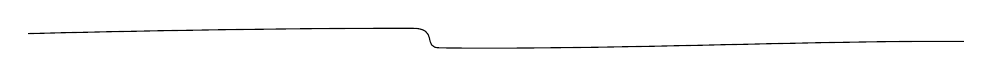
\begin{tikzpicture}[x=.98\linewidth,y=1ex]\draw (0,0) .. controls (.18,.35) and (.32,.45) .. (.41,.45) .. controls (.44,.45) and (.42,-1.2) .. (.44,-1.2) .. controls (.63,-1.35) and (.83,-.6) .. (1,-.65);\end{tikzpicture}}
\par\noindent\uline{For reference}

\diagram{\resizebox{\linewidth}{!}{\begin{tikzcd}[ampersand replacement=\&,column sep=2.2em,row sep=0pt,cells={nodes={inner sep=0pt}}]
{\left.\begin{array}{@{}l@{}}
\otimes\ \text{Resolution of singularities.}\\[.8ex]
\otimes\ \text{Cohomological purity.}
\end{array}\right\}}
\arrow[r,Rightarrow,yshift=1.1em]
\arrow[r,Rightarrow,yshift=-1.2em]
\& {\begin{array}{@{}l@{}}
\text{local duality}=\text{biduality,}\\[-.3ex]
\qquad\text{for the étale topology}\\[.8ex]
\text{finiteness theorem for \unsure{morphism|morphisms}}\\[-.3ex]
\qquad\text{\tikz[baseline=(fin.base)]{\node[inner sep=2pt] (fin) {\inserted{of finite type}};\draw ([yshift=-2pt]fin.north east) .. controls +(-.2,.05) and +(.2,0) .. (fin.north west) .. controls +(-.15,-.1) and +(-.1,0) .. (fin.south west) -- ([xshift=-8pt]fin.south east) .. controls +(.2,0) and +(0,-.1) .. (fin.north east);}}\\[-.3ex]
\text{and so on and so on}
\end{array}}
\end{tikzcd}}}

Regu\(\overset{\text{\scriptsize ?}}{\text{la}}\)r base change \inserted{in cohomology.}

Cohomological dimension of affine morphisms.

$\otimes$ Grauert-type finiteness \unsure{theorem|theorems}.

$\otimes$ Theories \deleted{\unsure{rigid|rigid}} of rigid-analytic type.

Questions in SGA 1962

\figure{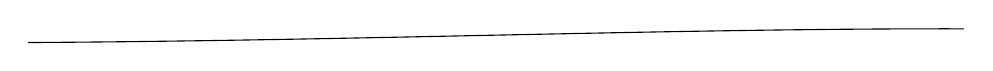
\begin{tikzpicture}[x=.98\linewidth,y=1ex]\draw (0,0) .. controls (.35,.15) and (.7,1.2) .. (1,1.15);\end{tikzpicture}}

\shortstack{23)\\[-.5ex]\scriptsize$\times$} Chow theory for \deleted{\unsure{arbitrary|arbitrary} regular} Schemes having an ample invertible sheaf (rational equivalence \unsure{of the|of}\unsure{,} cycles). The inverse image under $f:X\to Y$ must be defined, under the sole condition that $Y$ be regular.

\tikz[baseline=(num.base)]{\node[draw,circle,inner sep=.7pt] (num) {\shortstack{24\\[-.5ex]\scriptsize$\times$}};}
\margin{Negative answer by Griffiths to question 1\textsuperscript{o}}% slanted
\hspace{.4em}\inserted{1\textsuperscript{o}} On a smooth connected projective variety of dimension $3$ over $k$ an \unsure{algebraically|algebraically|algebraically} closed field, is a $1$-cycle numerically equivalent to $0$ $\tau$-equivalent to zero ? \inserted{In dimension $4$, cycles of dimension $2$ numerical equivalence $=$ homological equivalence ??\unsure{,|'}}
% archive sheet number: 3
\normalmarginpar
